\chapter{Intégration Continue}
\label{chap:integrationcontinue}

\section{Histoire}
La notion \textit{Intégration Continue} etait mentionné dans un livre de Grady Booch en 1994 pour la première foi\footnote{\cite{boochooad}}. Il parlait d'une intégration continue par des publications interne et chaque publication apporte l'application plus proche à la version finale.

La prochaine foi que l'intégration continue était sous les feux de l'actualité était avec la publication des concepts de \textit{Extreme Programming} en forme d'un livre en 1999.
Là inclue est l'idée d'avoir une machine dédié à l'integration du code et les pairs de developpeurs reunissant, integrant et testant le code source après chaque changement.\footnote{\cite{robertshistory}}

Une autre personne qui a gravé la notion \textit{Intégration Continue} est Martin Fowler. Il a publié un article sur le sujet en 2000 et revisé celui-ci six ans plus tard.\footnote{\cite{fowlerci}} Dans cet article il essayerait de donner une definition de l'IC et des meuilleures pratiques. Martin Fowler travaillait chez ThoughtWorks l'entreprise responsable pour la publication du première serveur d'\textit{Intégration Continue} "Cruise Control". Il est souvent cité comme personne-clé si on parle de l'IC.

Le premier livre publié sur la matière était "Continous Integration"\footnote{\cite{duvallconint}} en 2007. Naturellement il y a beaucoup d'autre livres traitant des technologie ou outils concrètes. Aujourd'hui le plus part d'entreprises implementes quelques ou tous les aspects de l'IC.

\nocite{wikici}
\newpage

\section{Aperçu}
Pour pouvoir comprendre le concept de base de l'Intégration Continue il est necessaire de connaitre le processus de development logiciel ordinaire. L'Intégration Continue n'éxige pas de méthode de gestion de projets specifique mais est souvent utilisé avec des approches agiles, car elle les complètent parfaitement. Voici un diagram d'un processus pareil. \footnote{Source http://www.techtipsnapps.com/2015/04/most-successful-software-development.html}

\begin{figure}[H]
	\centering
		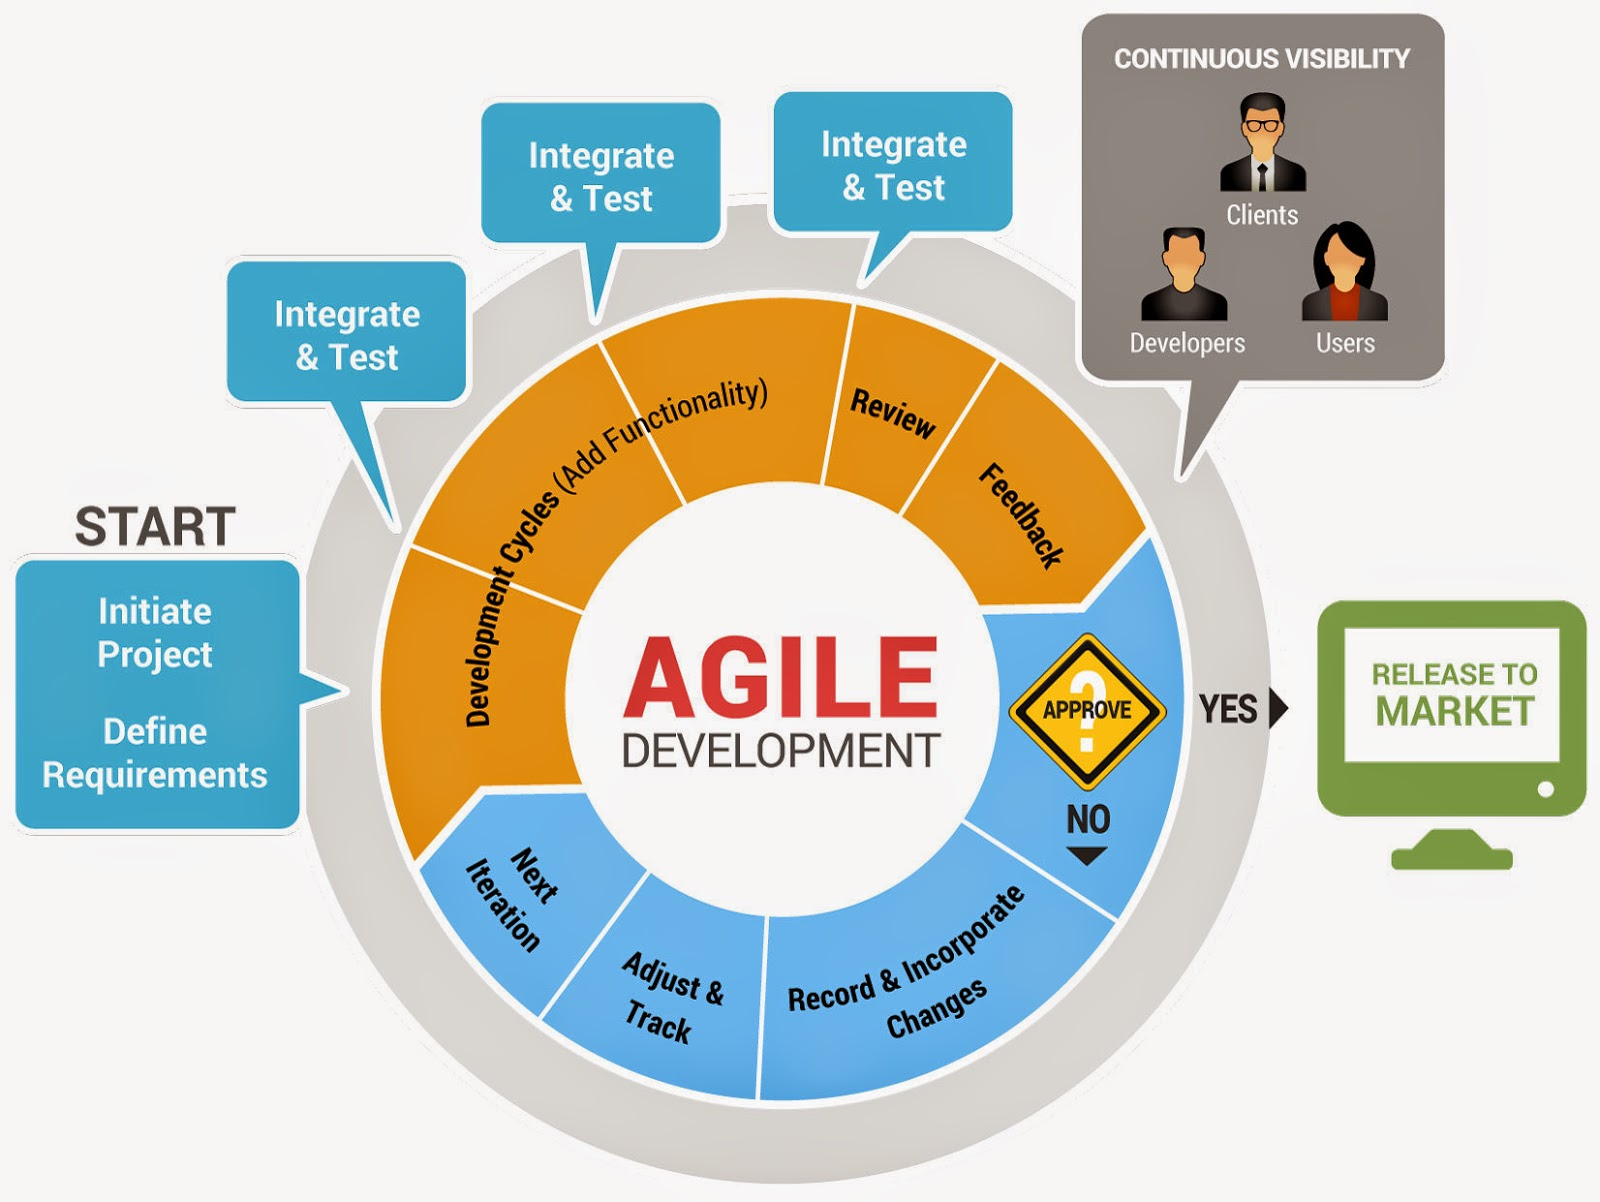
\includegraphics[scale=0.25]{bilder/agile_methodology}
	\caption{Processus de developpement logiciel}
	\label{fig:processus}
\end{figure}

L'idée principale de L'IC est d'automatiser des devoirs ou d'offrir de l'aide pendants les étappes de developpment. Pendant presque tous les projets de developpement on travaille en équippe. Tous les développeurs font des changements et ajoute de la fonctionnalité chaque jour. C'est pourquoi c'est necessaire de réunir ces changements regulièrement et de verifier si tous les composants marche et coopére comme voulu.\\\\
Ce processus de réunification s'appelle l'intégration. Si l'intégration est faite continuellement on parle de l'\textbf{Intégration Continue}. Mais une Intégration Continue à la lettre, chaque minute ou même en temp réel, n'est pas faisable ou aidant. C'est pour ça qu'une intégration executer au moins une foi par jour est suffisante.\\
De plus cette intégration doit être facile et automatisée, comme pousser un bouton. Tous le reste est controlé par le système IC. De plus la définition et l'étendue de l'IC est ouverte et pas strictement limité. Mais il y a quelques elements qui apparaissent dans tous les systèmes d'IC.
\newpage

\subsection{Architécture exemplaire}
Voici une architécture normale en travaillant avec un système d'Integration Continue.
\begin{figure}[H]
	\centering
		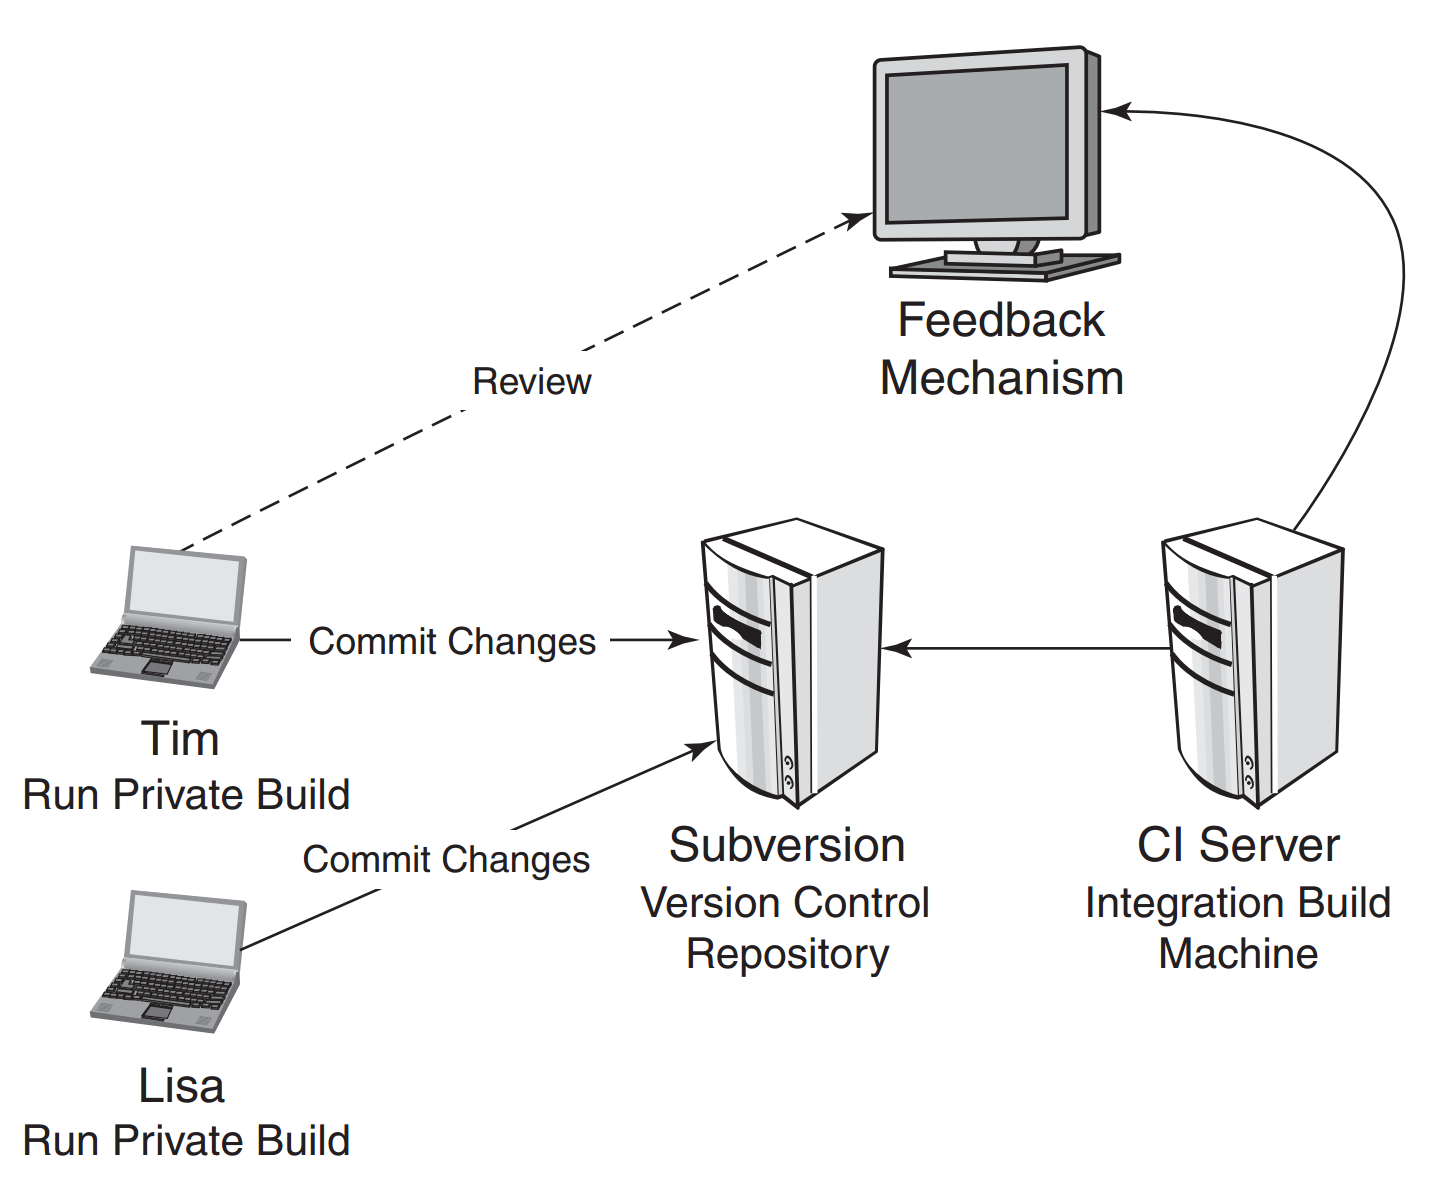
\includegraphics[scale=0.6]{bilder/architecture_exemplaire}
	\caption{Architécture exemplaire}
	\label{fig:processus}
\end{figure}

\textbf{Developpement locale}\\
Tous les developpeurs travaille sur ses machines privées ou des machines de l'entreprise. Avant d'ajouter de la fonctionalité la version la plus actuelle est téléchargé du dépot centrale. Après changer le code il est necessaire de faire un build et d'executer les testes unitaires. Si tout fonctionne les changements sont commit sur le dépot centrale.\\\\
\textbf{Dépot centrale}\\
Le dépot centrale est normalement un système de gestion de versions comme Subversion ou Git. Il est installé sur un serveur dédié. Tous les developpeur recoivent de l'accès pour commettre des changements là dessus. Ce faisant il est possible d'identifier qui a changé quoi en cas que quelque chose ne marche plus.\\\\
\textbf{Serveur de l'Intégration Continue} \\
Le serveur de l'Intégration Continue est la partie centrale du système. Il est aussi installé sur un serveur dédie, quelque foi sur la même machine que le dépot centrale. Le serveur IC controle reulièrement s'il y a une nouvelle version dans le dépot centrale. Si c'est le cas le serveur prends le code et démarre le processus d'intégration. Les étappes du processus doivent normalement être configurer une fois par projet. Quelques exemples pour des étappes possibles:
\begin{itemize}
\item Construction du code
\item Testes unitaires, testes d'intégration ou testes fonctionelle
\item Inspections
\item Création de sous-système ou deploiement
\end{itemize}
Si on inclue le deploiment dans le processus d'integration, il ne s'agit plus seulement de l'Intégration Continue, mais aussi du \textbf{Déploiment et de la Livraison Continue} (Continous Deployment, Continuous Delivery). 
\\\\
\textbf{Information en retour}\\
Après finir ce processus d'intégration les résultats des étappes est affiché sur un interface d'utilisateur centrale, souvent une page web. Pour toutes les étappes il est possible de configurer si l'échec de l'étappe amene l'échec du processus complet. Si il y a des erreurs les developpeurs et les personnes responsable peuvent être informer par des emails. Quelques entreprises installe des écrans dans les bureaux qui affichent les dernières résultats en temps réele.\\\\
Ces concepts seront discuter en détail pendant le prochain chapitre.
\section{Concepts de l'Intégration Continue}

\subsection{Construction continue}
\subsubsection{C/C++}
Le premier logiciel de construction était make, qui existes depuis 1976 (Stuart Feldman, Bell Labs). Sur les plateformes basé sur Unix make est encore utilisé pour construire des exécutables.
Pour construire une application avec make if faut fournir un fichier makefile qui contiens les instructions de compilation. Supposant on a un logiciel avec les fichiers: 

\lstinputlisting[language=C,caption={functions.h}]{../project/cpp_make_sample/functions.h}
\lstinputlisting[language=C,caption={factorial.c}]{../project/cpp_make_sample/factorial.c}
\lstinputlisting[language=C,caption={squared.c}]{../project/cpp_make_sample/squared.c}
\lstinputlisting[language=C,caption={main.cpp}]{../project/cpp_make_sample/main.cpp}

La commande pour compiler ce projet manuellement est:
$$g++\;main.cpp\;squared.cpp\;factorial.cpp\;-o\;hello$$
Pour un projet si petit c'est assez simple mais avec plus des fichiers ca se confus très vite.
Par exemple si on a beaucoup des dependences ou une application multi-plateforme c'est tres difficile de ne pas oublier quelque chose.
\newpage
\lstinputlisting[language=make,caption={Makefile sans variables}]{../project/cpp_make_sample/Makefile1.}
Si on regarde le fichier Makefile correspondant on voit que ca ne simplifie pas encore notre vie. Une prochaine étape est d'introduire des variables.
\lstinputlisting[language=make,caption={Makefile avec variables}]{../project/cpp_make_sample/Makefile2.}

Ce fichier est plus court et tres adaptable, mais il n est pas très lisible.
Utilisant l'outil cmake on peut générer les fichiers Makefile automatiquement (et autres fichiers de projet comme ".sln").
Dans le fichier CMakeLists.txt on définit quelles fichiers il faut compiler, quel sont les descendances...
\lstinputlisting[language=make,caption={CMakeLists.txt}]{../project/cpp_make_sample/CMakeLists.txt}


\subsubsection{Java}
Ant (Another neat tool) a apparu 2000, le premier logiciel de construction pour Java.
Aujourd'hui Ant et ses produits de concurrence Maven(2002) et Gradle(2012) sont inévitable si on utilise Java.
Dans ce moment environ 70 \% des développeurs Java utilisent Maven, 15 \% Ant et 15\% Gradle. Le concept est pareille comme en C++.


\subsection{Intégration continue de base de données}

Le plus part de logiciel utilisent une méthode pour persister des données, beaucoup de fois des bases de données. Le code source pour générer cette base de données doit être traiter comme tous le reste du code d'un projet. C'est necessaire qu'il soit aussi commit sur le dépot centrale et qu'on teste et fait des inspections là dessus.

\subsubsection{Automatisation de l'intégration}
Si le code de la base de données est aussi mis sur le dépot centrale, le processus de l'intégration de base de données peut être automatisé. Ce processus peut devenir assez complexe avec different environnements. Les serveurs, les noms d'utilisateur, les mots de passe ou bien les données de test ou de système peuvent differer pour chaque environnement.
\begin{figure}[H]
	\centering
		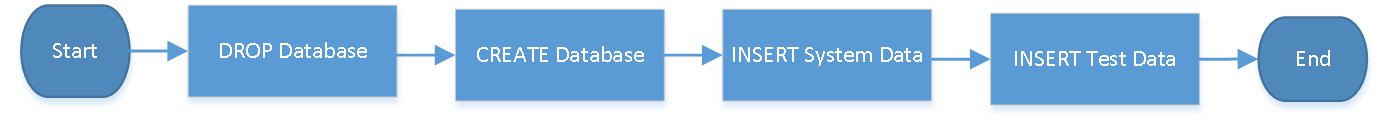
\includegraphics[scale=1]{bilder/database_integration}
	\caption{Processus de l'intégration de base de données}
	\label{fig:processus}
\end{figure}

C'est pour ca qu'une automatisation de ce processus est indispensable. Une automation est réalisé en insérant une section dans le script de construction uniquement pour les operations de l'intégration de base de données. L'interval et l'étendue de l'exécution de ce processus sont pas les mêmes pour tous les projets. Pour quelques projets ca pourrait être trop lourds de recrée la base de données à chaque changement sur le dépôt centrale. Avec l'outil de construction Maven et le plug-in "sql-maven-plugin" il est possible de definir quelle base de données est visé et quelles commandes sont exécuté. Voici une partie d'un tel script.\footnote{Pour l'éxample complète \cite{mvnsql}}

\lstinputlisting[language=XML]{./anhang/db_mvn_sql.xml}

\subsubsection{Instance de base de donnée locale}

Pour que cette approche fonctionne tous les développeurs doivent avoir l'autorisation de changer la base de données. Pour éviter des conflits pendant le développement tous les développeurs ont besoin d'une instance de cette base de données sur ses machines locales. Si on travaille avec une instance centrale à chaque changement il y a le danger de casser le code que quelqu'un d'autre est en train de développer.
\newpage


\subsection{Test continue}
Le premier principe de base pour des tests automatisés est "Fail fast" (Échouer vite).
C'est pourquoi on distingue trois types différents. Comme réglé d'or on  peut dire que les test unitaires prend des secondes, les tests d'intégration prend des minutes et les tests d'acceptation prend des heures.\nocite{artofunittesting}
\subsubsection{Tests unitaires}
Les tests unitaires vérifient le bon fonctionnement d' un bout de code. Pour les parties du code qui ne sont pas testable atomiquement on introduit des objets mock qui permettent des tests de fonctionnement vite et sans effets secondaires. 
\subsubsection{Tests d'intégration}
Pour tester l' interaction des parties testé avec les tests unitaires. Aussi l'interaction avec le système de fichier ou une base de données est testé ici. Apres les tests d'intégration les erreurs logiques doivent être éliminé.
\subsubsection{Tests d'acceptation automatisées}
Il y a différents types de test d' acceptation:
\begin{itemize}
 \item Tests d'interface utilisateur codé
 \\Pour ces tests il faut enregistrer des scénario. Les outils de test permettent de cliquer des boutons, entrer de text etc. 
 \item Tests de performance
 \\Ces tests montrent quelles parties du code prennent la plupart des ressources.
 \item Tests d'exploitabilité 
 \\Si le logiciel utilise une base de données on peut par exemple tester la vulnérabilité contre des attaques injection SQL.
 \item Tests de charge
 \\Par exemple: On a un magasin en ligne qui doit resister 100 utilisateurs à n'importe quel moment, testé avec les scenarios "login", "recherche des articles", "caisse", "login, ajouter, logout, login, effacer"
\end{itemize}





\subsection{Inspection continue}

La difference entre les testes et les inspections est que les inspections analyse la forme et la structure du code source et pas la fonctionnalité. Ces inspections sont introduit dans le processus de construction par différents plug-in. Les inspections ne remplacent pas les code review manuelles, mais dans ces reviews il y aura moins de défauts banale à traiter. Les objectifs des inspections sont engrèné là dessous.

\begin{enumerate}

\item \textit{Réduire la complexité du code source} \\ La complexité du code source peut être mesurée par la métrique "Cyclomatic Complexity Number (CCN)", qui compte le nombre de chemins distincts dans une méthode. Comme ça les endroits qui nécessite un changement peuvent être identifié (JavaNCSS, PMD \footnote{\citep{pluginpmd}}).

\item \textit{Determiner la dépendance} \\ Les métriques de couplage (Afferent/Efferent Coupling) et l'instabilité d'un package de logiciel peuvent être des indications à comme important on package est. Les packages qui sont utilisé très souvent il vaut mieux les tester très exactement (JDepend\footnote{\citep{pluginjdepend}}).

\item \textit{Imposer les standards de l'entreprise}\\ Dans chaque entreprise il y a des régles comment il faut écrire le code. Des examples très fréquemment sont que les variables n'ose pas avoir des noms trop courts et non-descriptive ou que les déclarations conditionel doivent toujours être écrit avec des parenthèses (PMD).
\item \textit{Reduire le code copié} \\ Le code source copié doit être avouer. Il y a des outils qui identifie des sections de code identique (PMD).

\item \textit{Determiner la couverture de code} \\ La couverture de code par les testes est une métrique qui aide à determiner quelles partie du code ont été negliger pendant écrire les testes (Cobertura\footnote{\citep{plugincobertura}}).

\end{enumerate}

\begin{figure}[H]
\centering
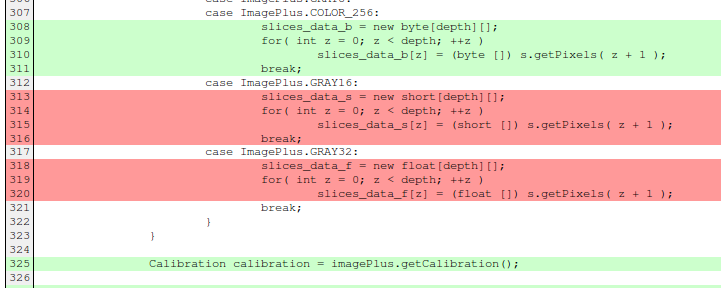
\includegraphics[width=15cm]{bilder/Coverage}
\caption{Couverture de code exemplaire} \cite{codecoverage}
\label{fig:coverage}
\end{figure}


\subsection{Information en retour continue}

Pendant le processus de construction c'est indispensable de savoir ce que se passe. Chaque etape de construction doit fournir des informations à tout-le-monde affecté. Classiquement c'est réalisé par envoyer un courriel. Les possibilités plus modernes sont des plug-ins directement dans l'environnement de développement(Team Explorer for TFS intégré dans Visual Studio), dans une application de online-chat(TravisCI native, TeamCity, Jenkins avec plugins), comme notification sur l'ordiphone ou dans le système d exploitation(Native dans Windows 10 ou avec differents apps tierce partie)...





\newpage
\subsection{Déploiement continue}

Le déploiement continue est un moyen pour délivrer la version actuelle aux utilisateurs immédiatement. Si un développeur fait un changement, la construction est initié automatiquement. Après ca les testes unitaires sont exécuté. Si tout les tests sont verts le développeur es informé et l'exécution des testes d'acceptation automatisées commence. Si la fonctionnalité du logiciel est assuré une nouvelle version est déployé immédiatement.


\begin{figure}[H]
\centering
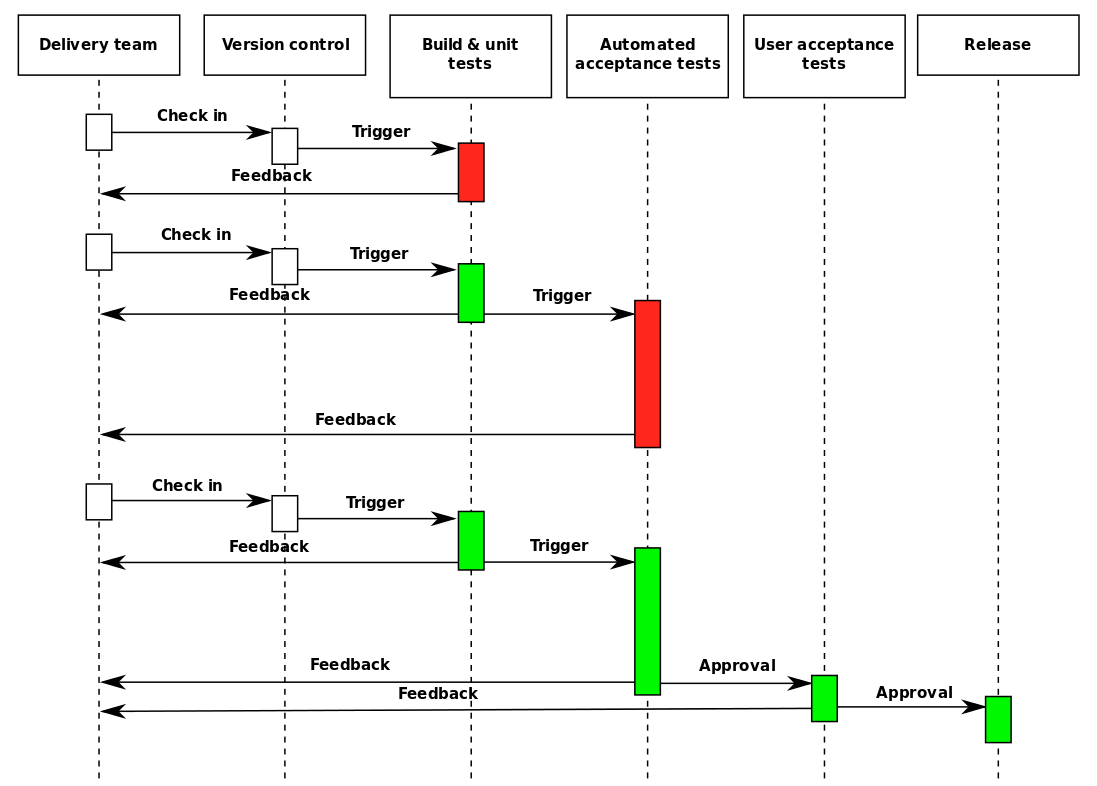
\includegraphics[width=15cm]{bilder/Continuous_Delivery}
\caption{Graphique déploiement continue}\cite{wikicd}
\label{fig:continousdelivery}
\end{figure}





\clearpage

\section{Motivation et bénéfices}

La raison principale pour utiliser l'IC est de garantir le succès et le déroulement d'un projet de développement de logiciel sans accroc. Dans tous les projets il y auras des problèmes et dans tous les logiciels il y auras des bogues. Mais l'IC aide à minimiser l'impact negatif que cettes erreurs ont.

De plus l'IC fait possible d'automatiser des processus ennuyeux, répétitif et sensible aux défauts. Par ça on peut économiser du temps et de la monnaie et les développeur se peuvent concentrer sour ce qu'ils aiment faire.

\subsection{Éviter des risques}
En dessous vous trouvez quelques risques que l'IC aide à éviter, mais seulement si la méthodologie est appliquée correctement (\nameref{sec:meuilleurespratiques}).\footnote{\cite[p39]{duvallconint}} 
\subsubsection{Logiciel pas déployable}
Si on fait l'integration d'un système seulement à la fin du projét, la probabilité de ne pas être capable à déployer et dérouler le logiciel pour le client est très haute. Des énonces comme "Mais ça marche sur ma machine" sont très connues. Des raisons pour cela peuvent être des configurations manquantes ou differentes sur la machine cible, ou même des dépendances qui n'ont pas été inclus pour le deploiement. Naturellement si le code source ne compile pas, le logiciel ne peut non plus être déroulé.

En commettre, construire et deployer le logiciel souvent ce risque peut être diminuer. En faisant ça on a la certitude d'avoir au moins un logiciel qui marche partiellement.
\subsubsection{Découverte tarde des erreurs}
Par l'exécution des testes automatiques pendant le processus de construction des erreurs dans le code source peuvent être decouvrit tôt. De plus il est aussi possible de determiner la couverture du code par les tests. Surement la qualité des testes doit être bonne.
\subsubsection{Manque de visibilité du projet}
L'opération d'un serveur d'IC crée la clarté de l'état actuelle de l'application et aussi de sa qualité. Si il y a un problème avec les changements derniers toutes les personnes responsables seront contacter. Si une nouvelle version a été deployé pour le testing, les personnes testant le logiciels seront aussi automatiquement informé.

Il existe mêmes des outils qui font la visualisation du projet possible, par génerant des diagrams UML du code courant. Ca aide à donner un apercu pour des developpeurs nouvels et garantis une documentation toujours actuel du projet.
\subsubsection{Logiciel de basse qualité }
Le code source qui ne suit pas les règles de programmation, le code source qui suit une architecture different ou le code redondant pourrant devenir des erreurs dans le futur.
Par executant des testes et des inspections regulièrement ces dérogations peuvent être trouvé avant de devenir un vrai problème.
\clearpage

\section{Meuilleures pratiques}
\label{sec:meuilleurespratiques}

En dessous vous trouvez quelques pratiques qui aident à optimiser l'efficacité d'un système d'IC.\footnote{CI and You \cite[p~47]{duvallconint}}

\begin{enumerate}

\item \textbf{Étendue de l'implementation (Scope of implementation)}\\
Avant de commencer l'implementation d'un système de l'IC c'est absolument necessaire de savoir de quelles composants on a besoin. Pas tous les projets necessite les mêmes mesures, ça dépends fortement de la taille, de la complexité du projet et du nombre de personnes impliqué. 
De plus il est conseillé de ne pas configurer tous les composant en même temps, mais de faire ça par étappes (p.ex. build, testing, review, deploy). 

\item\textbf{Commettre le code souvent (Commit code frequently)}\\
Il est conséillé de commettre le code source au moins une foi par jour. Essaie de fragmenter le travail dans des morceaux petits et de commettre après chaque partie.

\item\textbf{Ne jamais commettre du code non-compilable (Dont commit broken code)}

\item\textbf{Éviter le code non-fonctionnnant (Avoid getting broken code)}

\item\textbf{Faire la construction localement (Run private builds)}

\item\textbf{Découpler le processus de construction de l'IDE (Decouple build process from IDE)}\\
L'IDE peut faire des pas dans le processus de construction qui ne sont pas transparent pour le developpeur ou les developpeur utilises des different IDE. C'est pour ça que la construction doit être possible et fait à dehors d'une IDE.

\item\textbf{Reparer des constructions non-fonnctionnant immédiatement (Fix broken builds immediately)}\\
Si quelque chose ne marche pas la reparation doit avoir la première priorité.

\item\textbf{Écrire des testes automatisé (Write automated developer tests)}

\item\textbf{Tous les testes doivent réussir (All tests and inspections must pass)}\\
Si on ignore des testes qui ne réuissent pas on diminue la visibilité du projét.

\item\textbf{Des constructions vite (Keep builds fast)}\\

\end{enumerate}



